\begin{frame}
\frametitle{Day 20: Pulse Propagation}

You have a collection of modules that can send and receive high or low pulses connected together. There are three main types:
\begin{itemize}
    \item Flip-flop modules $(\%)$, when receiving a low pulse, flip their internal state between sending a high pulse or a low pulse, defaulting to high.
    \item Conjunction modules $(\&)$ remember the most recent pulses from each input, defaulting their memory to low - if all pulses in memory are high, it sends a low pulse, else high.
    \item There is a button/broadcast module that sends a low pulse to all of its destination modules.
\end{itemize}\vfill

Pulses are processed in the order they are sent.

\end{frame}

\begin{frame}
\frametitle{Day 20: Button}

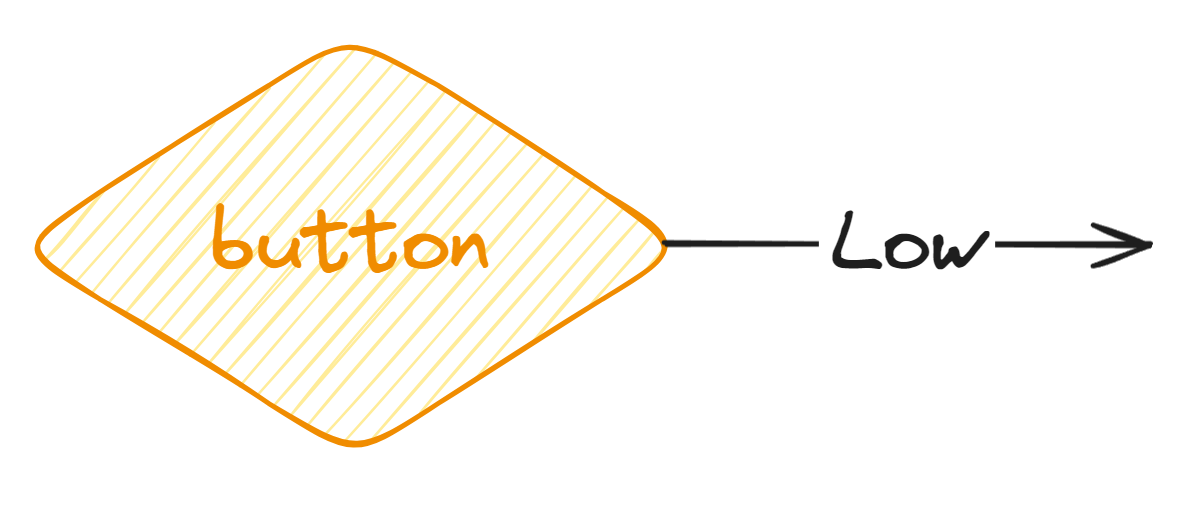
\includegraphics[width=\textwidth]{Day20Button}

\end{frame}

\begin{frame}
\frametitle{Day 20: Flip Flop}

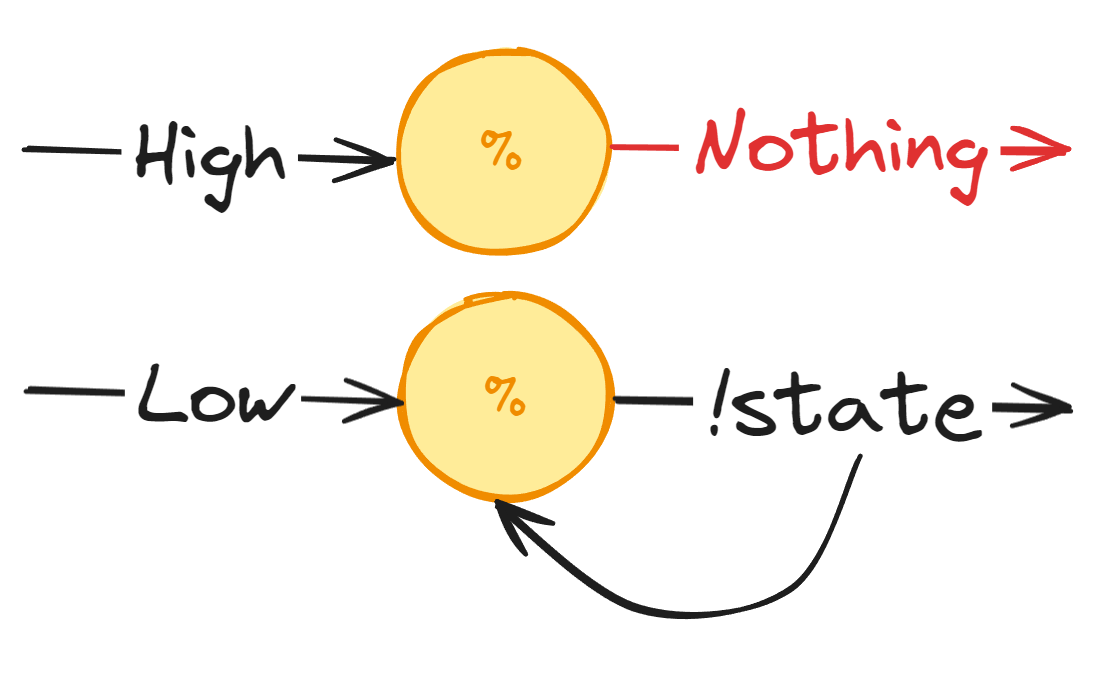
\includegraphics[width=\textwidth]{Day20FlipFlop}

\end{frame}


\begin{frame}
\frametitle{Day 20: Conjunction}

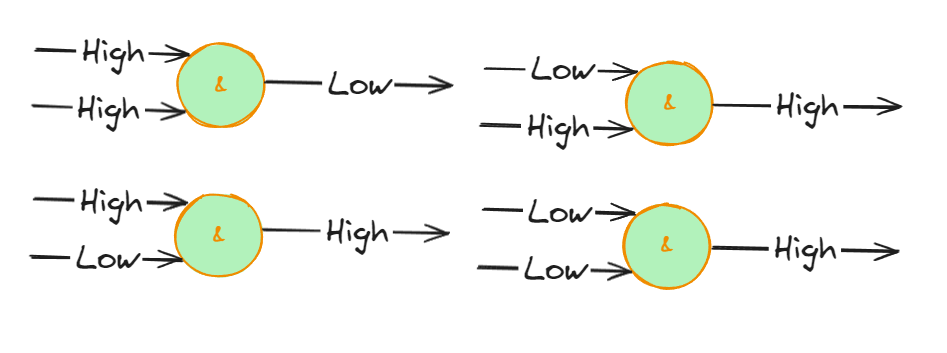
\includegraphics[width=\textwidth]{Day20Conjunction}

\end{frame}

\begin{frame}[fragile]
\frametitle{Day 20: Example}

\begin{center}
\begin{minipage}{0.45\textwidth}
\begin{center}
\begin{verbatim}
btn -> a, b, c
%a -> b
%b -> c
%c -> inv
&inv -> a        
\end{verbatim}
\end{center}
\end{minipage}
\begin{minipage}{0.45\textwidth}
\begin{center}
\begin{verbatim}
btn -low-> a
btn -low-> b
btn -low-> c
a -high-> b
b -high-> c
c -high-> inv
inv -low-> a
a -low-> b
b -low-> c
c -low-> inv
inv -high-> a        
\end{verbatim}
\end{center}
\end{minipage}
\end{center}

\end{frame}

\begin{frame}[fragile]
\frametitle{Day 20: Example Cont.}

\begin{center}
\begin{verbatim}
                   a:1, b:1, c:1, inv:[c:0]
btn -low-> a       a:0, b:1, c:1, inv:[c:0]
btn -low-> b       a:0, b:0, c:1, inv:[c:0]
btn -low-> c       a:0, b:0, c:0, inv:[c:0]
a -high-> b        a:0, b:0, c:0, inv:[c:0]
b -high-> c        a:0, b:0, c:0, inv:[c:0]
c -high-> inv      a:0, b:0, c:0, inv:[c:1]
inv -low-> a       a:1, b:0, c:0, inv:[c:1]
a -low-> b         a:1, b:1, c:0, inv:[c:1]
b -low-> c         a:1, b:1, c:1, inv:[c:1]
c -low-> inv       a:1, b:1, c:1, inv:[c:0]
inv -high-> a      a:1, b:1, c:1, inv:[c:0]
\end{verbatim}
\end{center}

\end{frame}

\begin{frame}
\frametitle{Day 20: Part 1}

After 1,000 button presses, how many pulses were sent?\vfill

Simulation go brrr

\end{frame}

\begin{frame}
\frametitle{Day 20: Part 2}

We want to know how many button presses are required to send a single low pulse to module rx.\vfill

Simulation go brrr... for a long time. A bit over 270,000 times longer. Clearly, computation is not the way to go.\vfill

\end{frame}

\begin{frame}
\frametitle{Day 20: Graph (Unified)}

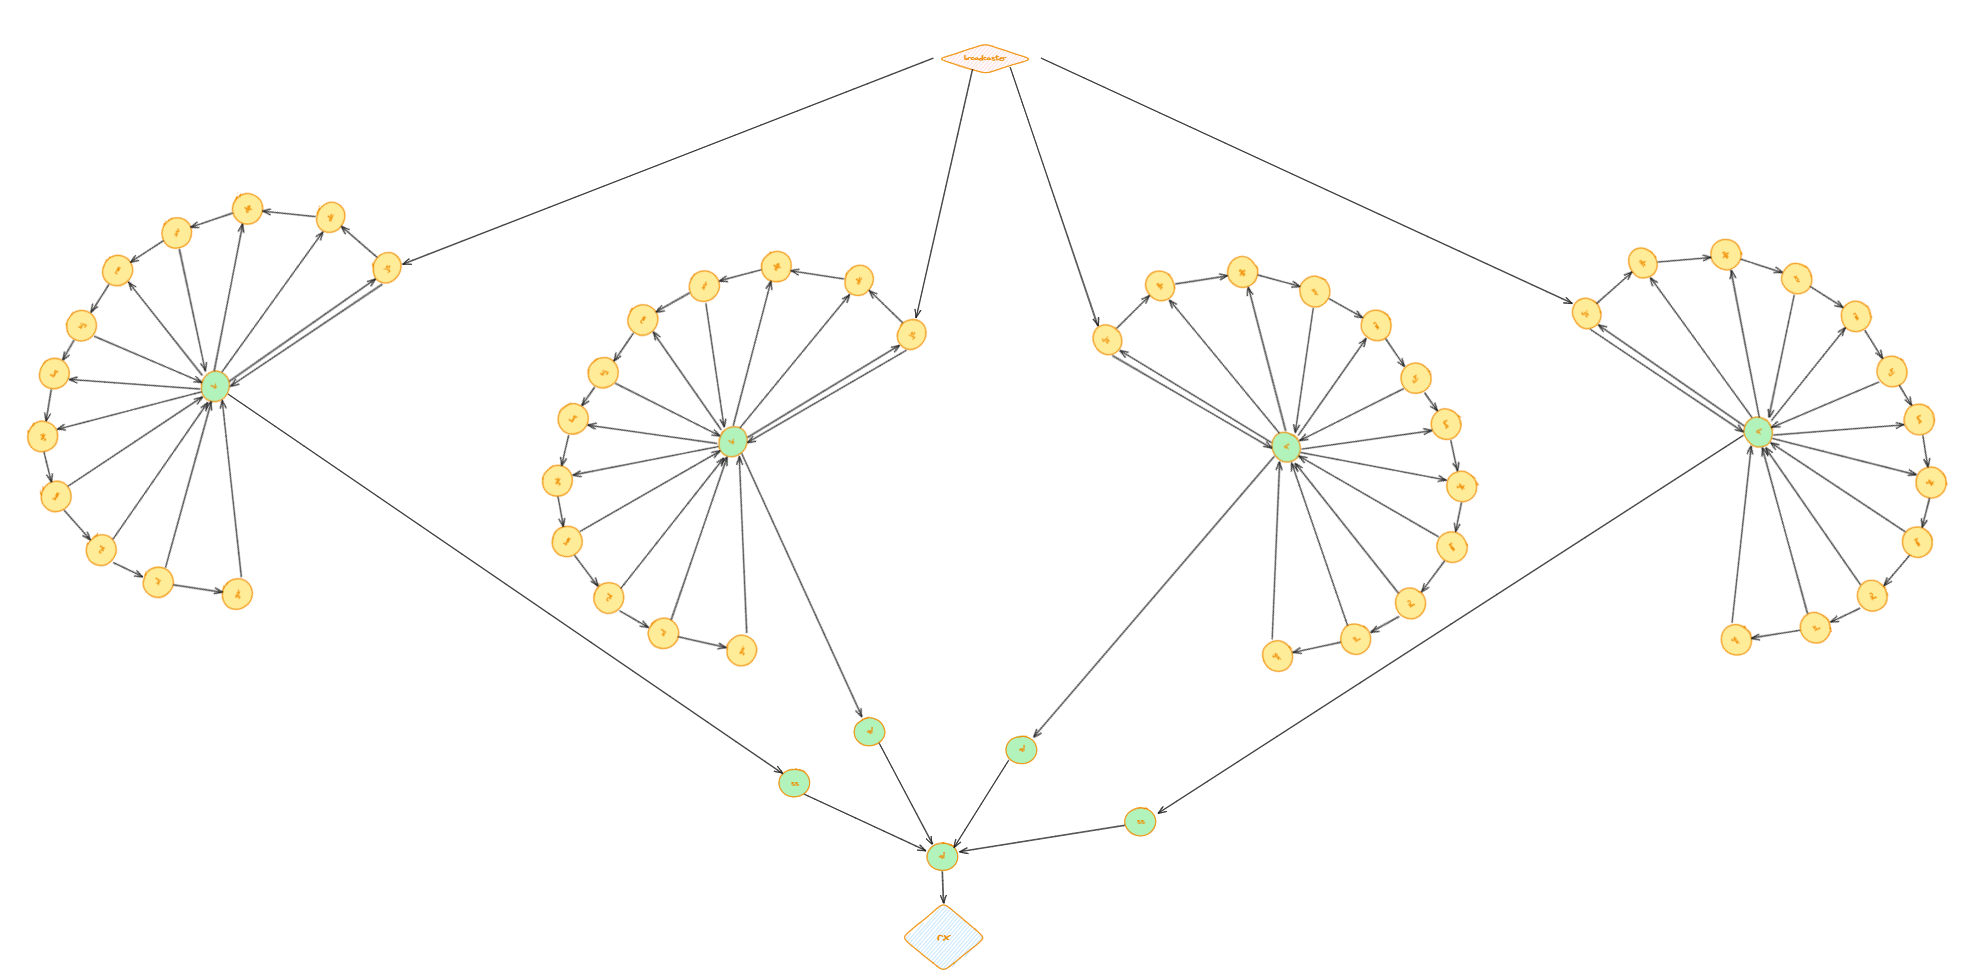
\includegraphics[width=\textwidth]{Day20GraphUnified}

\end{frame}

\begin{frame}
\frametitle{Day 20: Graph (Separate)}

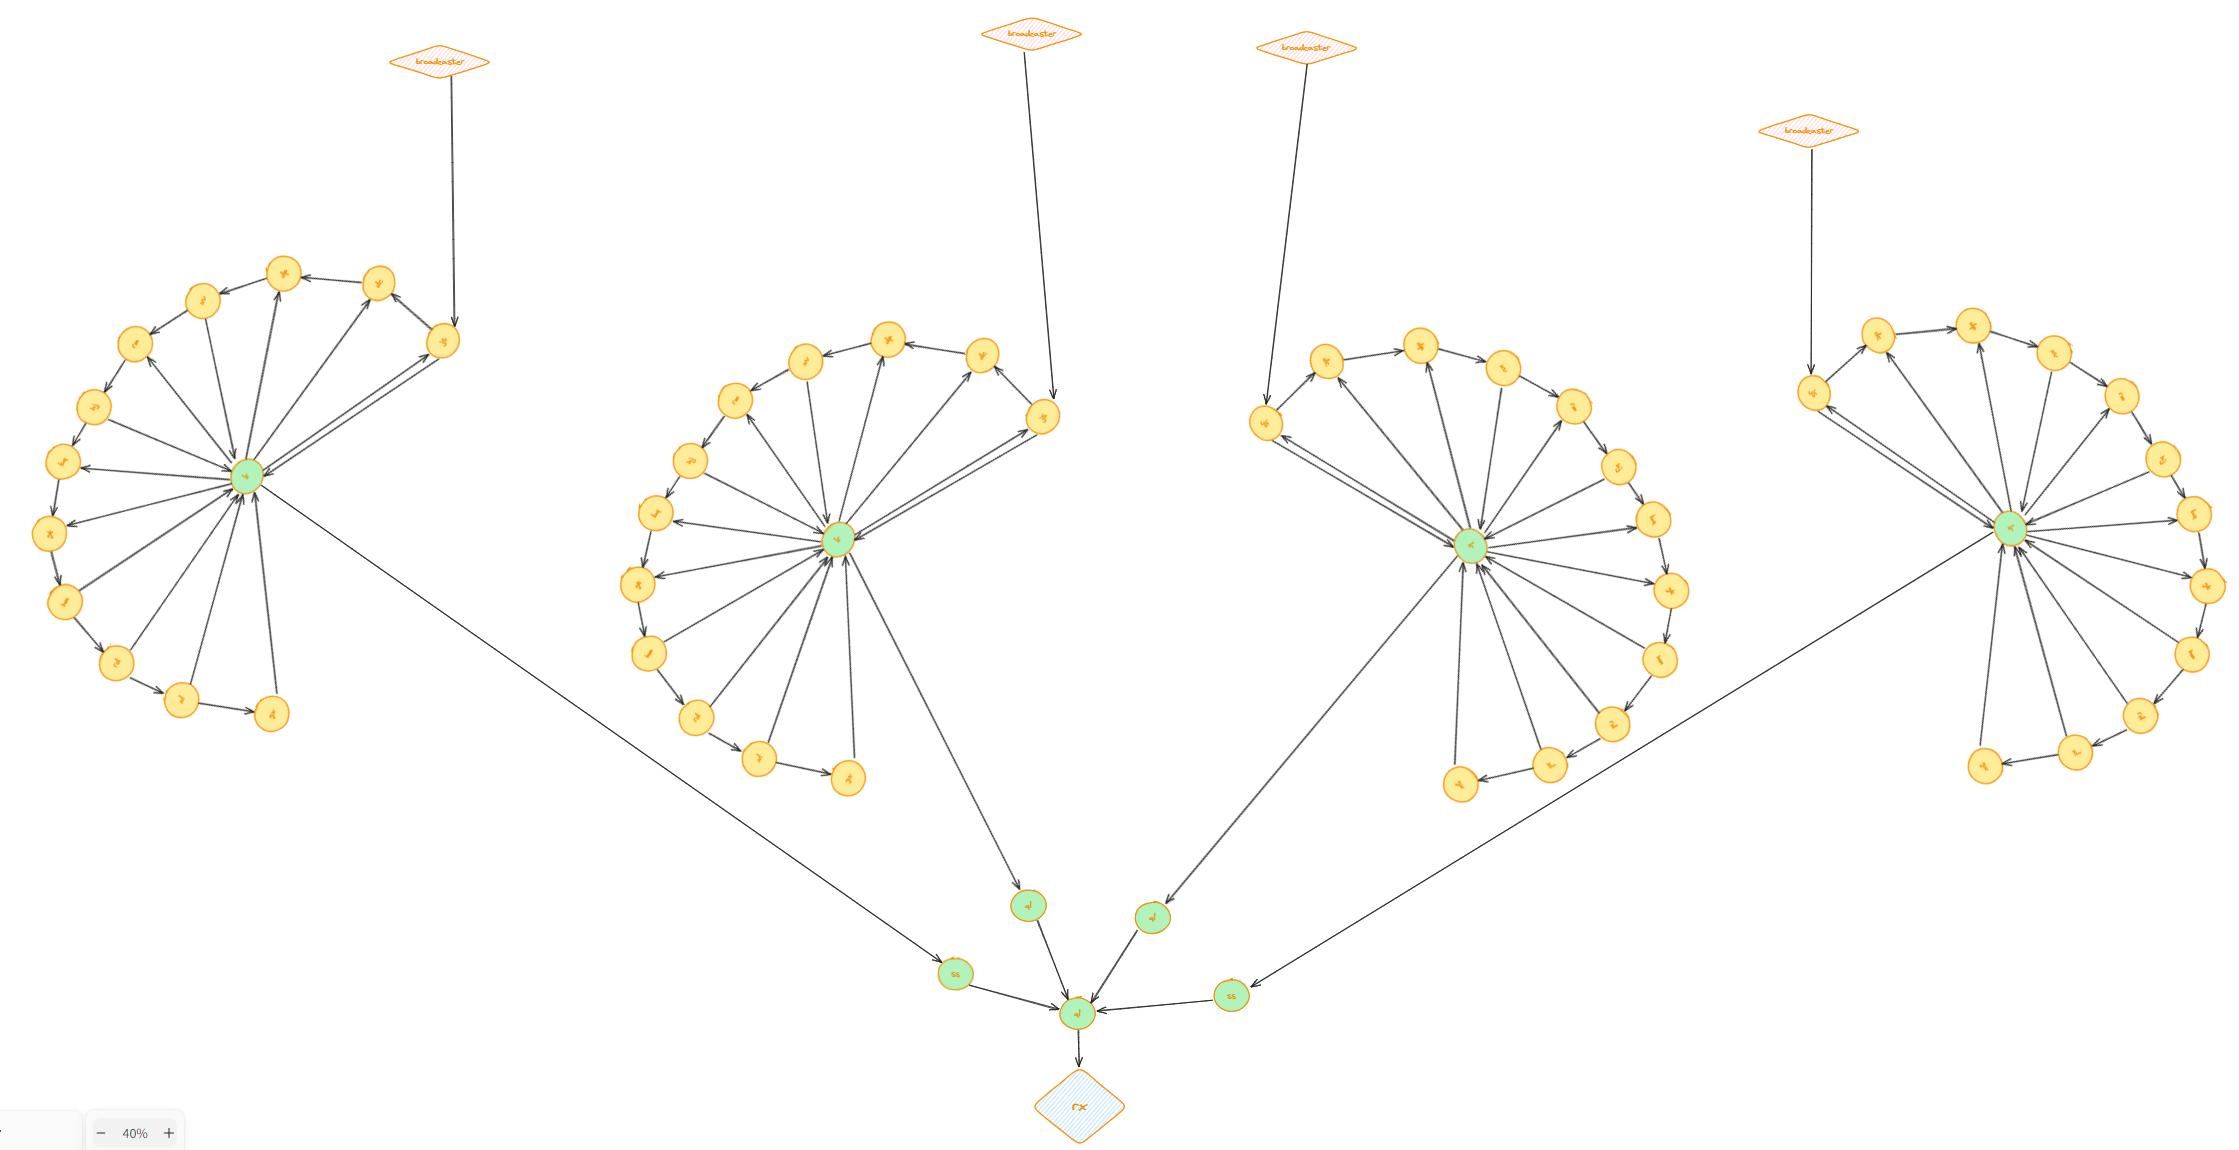
\includegraphics[width=\textwidth]{Day20GraphSeparate}

\end{frame}

\begin{frame}
\frametitle{Day 20: Graph (Black Box)}

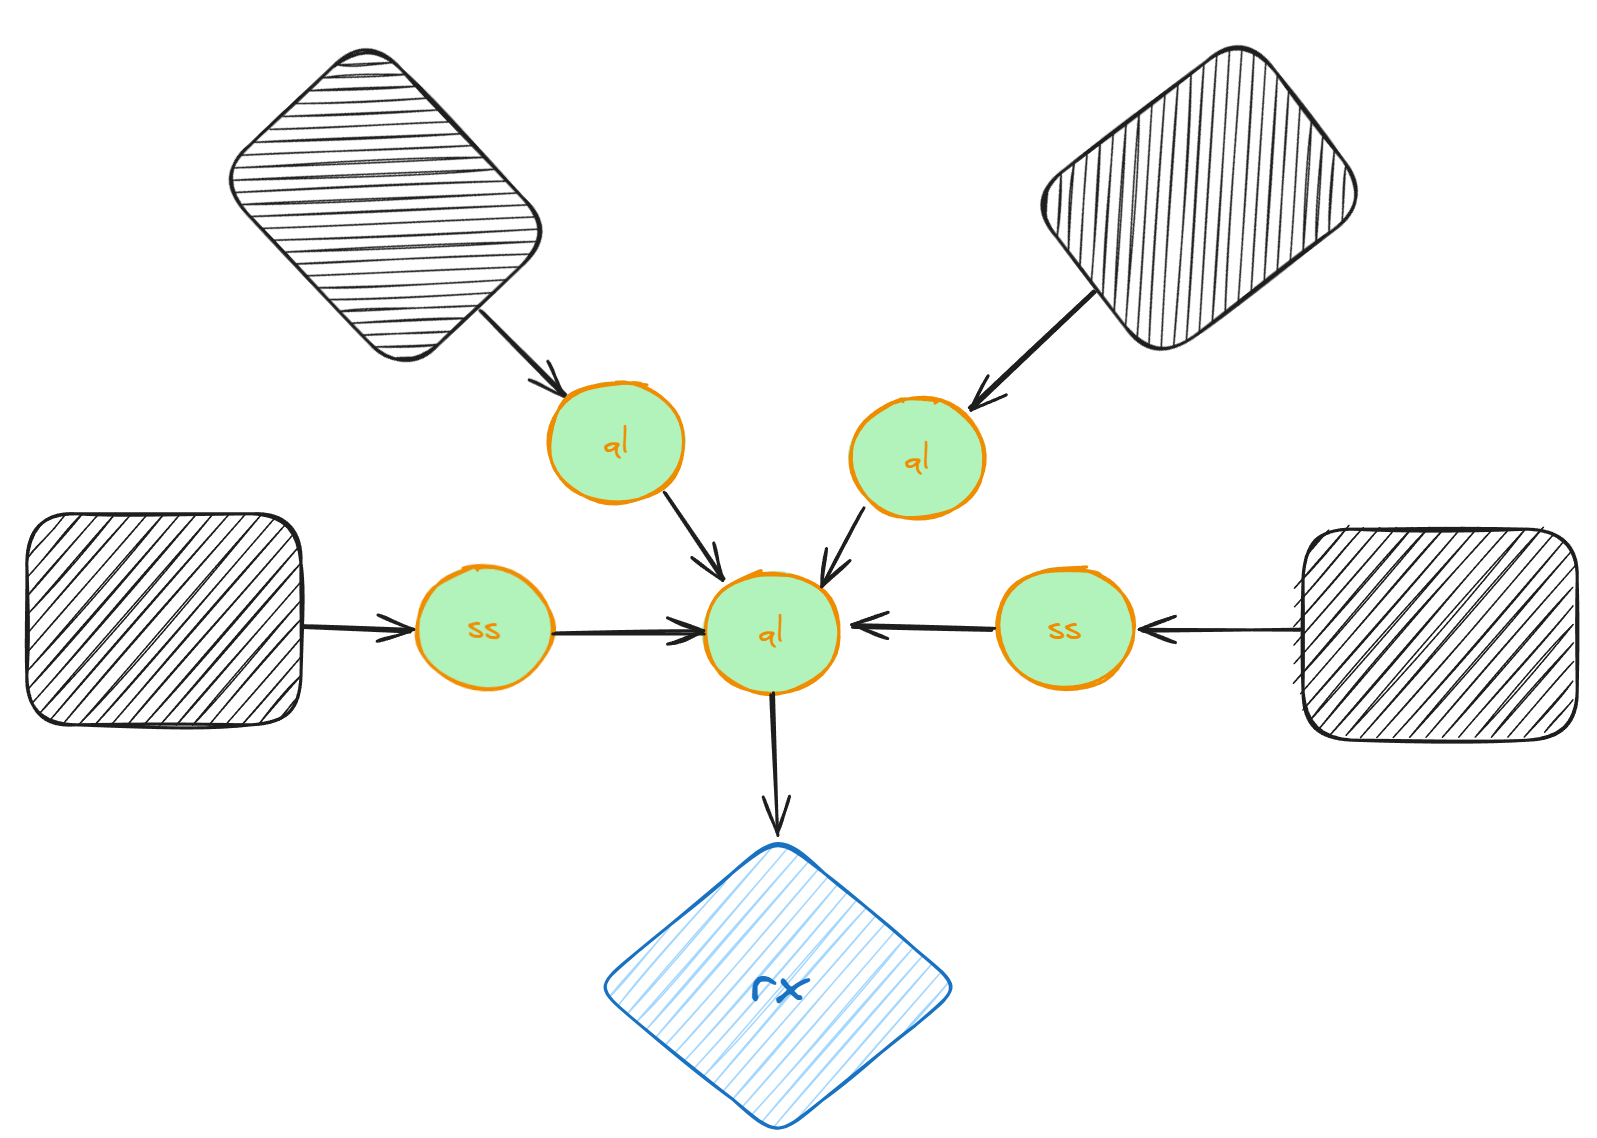
\includegraphics[width=\textwidth]{Day20BlackBox}

\end{frame}

\begin{frame}
\frametitle{Day 20: Break It Down}

Module rx only receives input from dr.\linebreak
Module dr only receives input from qt, qb, ng, mp.\linebreak
Modules qt, qb, ng, mp each receive input from a unique subgraph.\vfill

Each subgraph can be "solved" independently.

\end{frame}